\section{Tema 3: Conservación de la masa}
\subsection{Teorema del transporte de Reynolds}
Se parte de una función genérica $\Phi=f(\vec{r},t) $
\begin{figure}[H]
	\centering
	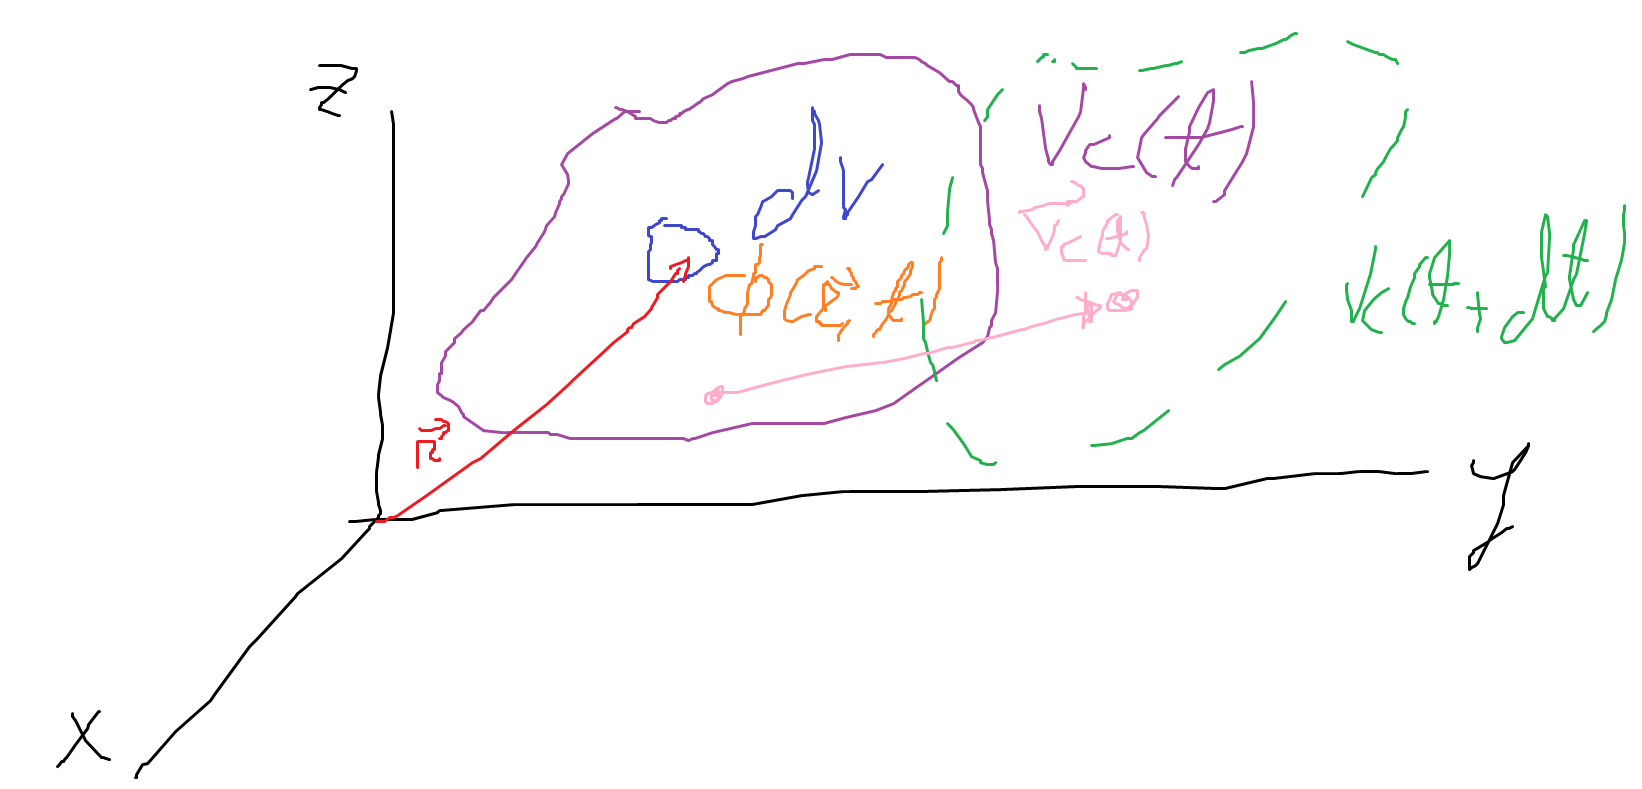
\includegraphics[width=0.7\linewidth]{imagenesTema3/magnitudesReynolds}
	\caption{Evolución de una magnitud en un volumen fluido.}
	\label{fig:magnitudesreynolds}
\end{figure}

Por definición de derivada:
\[\frac{d}{dt}\iiint_{V_c(t)} \Phi(\vec{r},t) \,dV=\lim_{\Delta t \to 0} \left[\iiint_{V_c(t+dt)} \Phi(\vec{r},t+dt) \,dV-\iiint_{V_c(t)} \Phi(\vec{r},t) \,dV\right]\]

Se hace el desarrollo de Taylor en t del primer término:
\[\frac{d}{dt}\iiint_{V_c(t)} \Phi(\vec{r},t) \,dV=\iiint_{V_c(t)} \frac{\partial}{\partial t}\Phi(\vec{r},t) \,dV+\lim_{\Delta t \to 0} \frac{1}{\Delta t}\left[\iiint_{V_c(t+dt)} \Phi(\vec{r},t) \,dV-\iiint_{V_c(t)} \Phi(\vec{r},t) \,dV\right]\]

Como solo se estudia la velocidad de compresión o expansión del fluido en la dirección de la superficie de control:
\[dV=\vec{v}_c\cdot\vec{n}dS\Delta t\]

Por tanto:
\begin{equation} \label{eq:1}
\frac{d}{dt}\iiint_{V_c(t)} \Phi(\vec{r},t) \,dV=\iiint_{V_c(t)} \frac{\partial}{\partial t}\Phi(\vec{r},t) \,dV+\oiint_{S_c(t)} \Phi(\vec{r},t)\vec{v}_c\cdot\vec{n} \,dS
\end{equation}

De manera similar se puede aplicar esta deducción a un volumen fluido:
\begin{equation} \label{eq:2}
\frac{d}{dt}\iiint_{V_f(t)} \Phi(\vec{r},t) \,dV=
\red{\underbrace{\black\iiint_{V_f(t)} \frac{\partial}{\partial t}\Phi(\vec{r},t) \,dV}_{\text{Variación local}}}
\black+
\red{\underbrace{\black\oiint_{S_f(t)} \Phi(\vec{r},t)\vec{v}\cdot\vec{n}\,dS}_{\text{Variación convectiva}}}
\black
\end{equation}

En un tiempo t* paramétrico tal que $V_c(t*)=V_f(t*)$ se cumple que
\[ \iiint_{V_c(t*)}\frac{\partial \Phi}{\partial t}\,dV\approx \iiint_{V_f(t*)}\frac{\partial \Phi}{\partial t}\,dV\]

Por tanto, si se hace la siguiente resta $(2)-(1)$. Se obtiene el Teorema de Reynolds aplicado a los problemas:

\[\frac{d}{dt}\iiint_{V_f(t)}\Phi(\vec{r},t)\,dV=\frac{d}{dt}\iiint_{V_c(t)}\Phi(\vec{r},t)\,dV+\oiint_{S_c(t)} \Phi(\vec{r},t)\left[(\vec{v}-\vec{v}_c)\cdot\vec{n}\right] \,dS\]



Si la magnitud $\Phi = \rho$ Se obtiene la ecuación de conservación de la masa en forma integral, que como en todo el volumen fluido no varia es igual a 0:

\[\frac{d}{dt}\iiint_{V_f(t)}\rho\,dV=\frac{d}{dt}\iiint_{V_c(t)}\rho\,dV+\oiint_{S_c(t)} \rho\left[(\vec{v}-\vec{v}_c)\cdot\vec{n}\right] \,dS=0\]

Para todo el volumen fluido:
\[\frac{d}{dt}\iiint_{V_f(t)} \rho \,dV=\iiint_{V_f(t)} \frac{\partial \rho}{\partial t} \,dV+\oiint_{S_f(t)} \rho\vec{v}\cdot\vec{n} \,dS=0\]

Si $V_f(t)\approx dV_f(t)$ entonces aplicando el teorema de gauss se llega a la ecuación diferencial de la masa o forma conservativa:

Teorema de Gauss:
\[\oiint_S \varphi \cdot \vec{n}\,dS=\iiint_V \vec{\nabla}\cdot\varphi\,dV\]

\[\lim_{dV \to 0}\left[\frac{\partial \rho}{\partial t} dV+\vec{\nabla}\cdot\left(\rho\vec{v}\right)dV\right]=0\]
\[\frac{\partial \rho}{\partial t} +\vec{\nabla}\cdot\left(\rho\vec{v}\right)=0\]
Término local de masa: 
\[\frac{\partial \rho}{\partial t}\]
Término convectivo de masa:
\[\vec{\nabla}\cdot\left(\rho\vec{v}\right)\]
